%
% CURVAS ELÍPTICAS
%
\section{Curvas Elípticas}

\subsection{Definição}
Curvas elípticas não são elipses. Elas têm esse porque são descritas por equações cúbicas, semelhantes às usadas para calcular a circunferência de uma elipse. Em geral, as equações cúbicas para curvas elípticas têm a forma
\begin{equation}
y^2 + axy + by = x^3 + cx^2 + dx + e \label{eq:11}
\end{equation}
onde \(a, b, c, d\) e \(e\) são números reais e \(x\) e \(y\) assumem valores nos números reais. Equações deste tipo são chamadas de \textit{equações de Weiestrass}. Para a nossa finalidade, é suficiente limitarmos na forma normal da equação de Weiestrass
\begin{equation}
y^2 = x^3 + ax + b \label{eq:12}
\end{equation}

Essas equações são consideradas cúbicas, ou de grau 3, pois o expoente mais alto que elas contém é um 3. Também incluído na definição de uma curva elíptica está um único elemento indicado por \(O\) e chamado de \textit{ponto no infinito} ou \textit{ponto zero}.

A Figura \ref{fig:curvas} apresenta alguns exemplos de curvas elípticas usando a forma normal da equação de Weierestrass.

\begin{figure}[h]
\centering
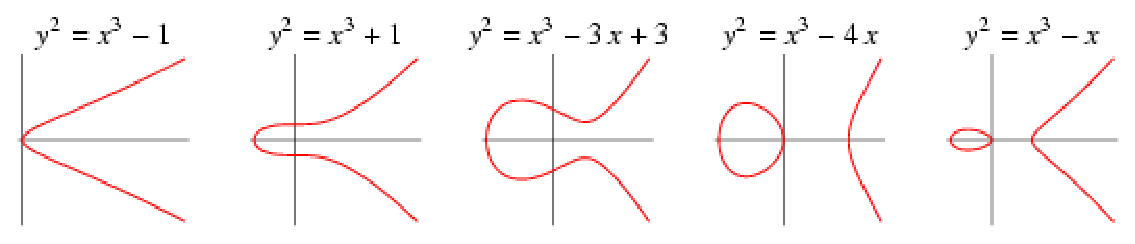
\includegraphics[scale=0.5, bb=0 0 529 101]{figuras/curvas.eps}
\caption{Exemplos de curvas elípticas}
\label{fig:curvas}
\end{figure}

Podemos mostrar que um grupo pode ser definido com base no conjunto E(\(a, b\)) para valores específicos de \(a\) e \(b\) na Equação \ref{eq:12}, desde que a condição a seguir seja atendida:
\begin{equation}
4a^3 + 27b^2 \neq 0 \label{eq:7}
\end{equation}

\subsection{Propriedades}
Uma importante característica da curvas elípticas é que existe uma forma natural de ``somar'' dois pontos produzindo um terceiro ponto. Para tanto, deve-se satisfazer a Equação \ref{eq:7}. No entanto, esta ``soma'' se refere à operação que combina dois pontos de maneira análoga da soma algébrica em alguns aspectos (é comutativa, associativa e existe um elemento identidade), mas bem diferente em outras formas.

Em termos geométricos, as regras para a adição podem ser indicadas da seguinte maneira: se três pontos em uma curva elíptica se encontram em uma linha reta, sua soma é \(O\). Por essa definição, podemos definir as regras da adição sobre uma curva elíptica:

\begin{figure}[h]
\centering
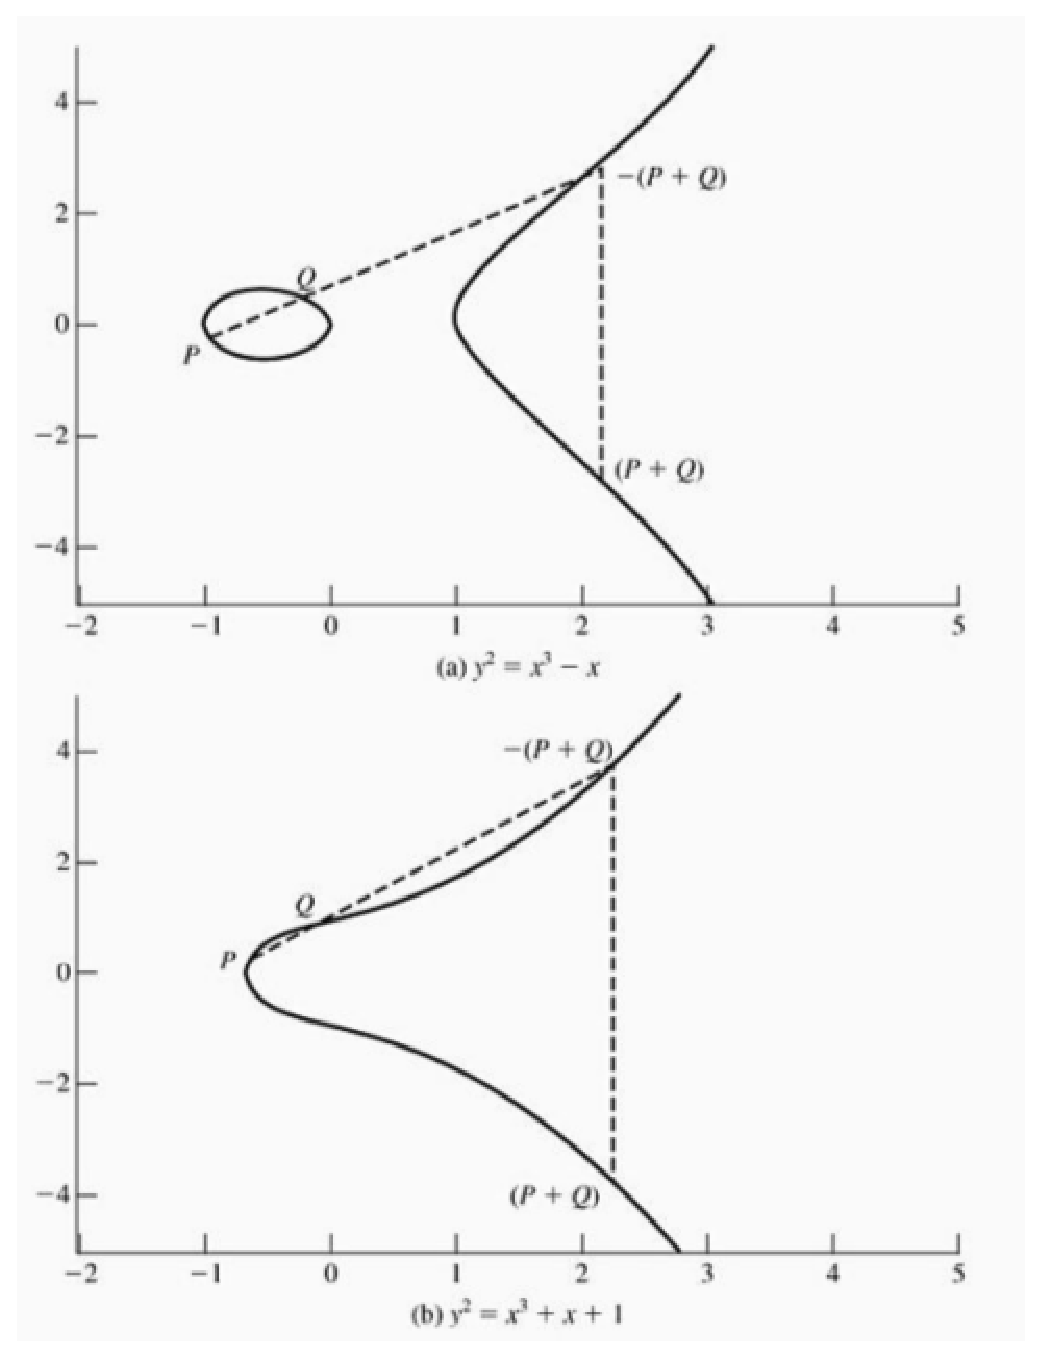
\includegraphics[scale=0.5, bb=0 0 484 636]{figuras/pontos_curva.eps}
\caption{Exemplos de soma de pontos em curvas elípticas}
\label{fig:pontos}
\end{figure}

\begin{enumerate}
	\item $O$ funciona como a identidade aditiva. Assim, $O = -O$; para qualquer ponto $P$ na curva elíptica, $P + O = P$. A seguir, consideramos $P \neq O$ e $Q \neq O$.
	\item O negativo de um ponto \(P\) é o ponto com a mesma coordenada \(x\), sem o negativo da coordenada \(y\); ou seja, se $P=(x,y)$, então $-P=(x,-y)$. Observe que esses dois pontos podem ser juntados por uma linha vertical. Observe que $P+(-P)=P-P=O$.
	\item Para somar dois pontos \(P\) e \(Q\) com coordenadas \(x\) diferentes, desenhe uma linha reta entre eles e encontre o terceiro ponto de interseção \(R\). Pode-se ver facilmente que existe um único ponto \(R\) que é o ponto de interseção (a menos que a linha seja tangente à curva em \(P\) ou \(Q\), quanto consideramos $R=P$ ou $R=Q$, respectivamente). Para formar uma estrutura de grupo, precisamos definir a adição sobre três pontos da seguinte forma: $P+Q=-R$. Ou seja, definimos $P+Q$ como sendo a imagem-espelho (com relação ao eixo \(x\)) do terceiro ponto da interseção. A figura \ref{fig:pontos}
	\item A interpretação geométrica do item anterior também se aplica a dois pontos, \(P\) e \(-P\), com a mesma coordenada \(x\). Os pontos são reunidos por uma linha vertical, que também pode ser vista como a interseção da curva no ponto infinito. Portanto, temos $P+(-P)=O$, coerente com o item (2).
	\item Para dobrar um ponto \(Q\), desenhe uma linha tangente e encontre o outro ponto da interseção \(S\). Então, $Q+Q=2Q=-S$.
\end{enumerate}

Com a lista de regras apresentada, pode-se se mostrar que o conjunto E(\(a, b\)) é um grupo abeliano. \cite{Stallings:2011}

\subsection{Adição de pontos}
Para dois pontos distintos $P = (x_P, y_P)$ e $Q = (x_Q, y_Q)$ que não são negativos um do outro, a inclinação da linha \(l\) que os junta é $\Delta = (y_Q - y_P)/(x_Q - x_P)$. Existe exatamente um outro ponto onde \(l\) cruza a curva elíptica, e esse é o negativo da soma de \(P\) e \(Q\). Após alguma manipulação algébrica, podemos expressar a soma $R = P + Q$ da seguinte forma:

\begin{eqnarray}
x_R &=& \Delta^2 - x_P - x_Q \\
y_R &=& -y_P + \Delta(x_P - x_R)
\end{eqnarray}

Também é preciso ser capaz de incluir um ponto em si mesmo: $P + P = 2P = R$. Quando $y_P \neq 0$, as expressões são

\begin{eqnarray}
x_R &=& \left(\frac{3x_P^2 + a}{2y_P}\right)^2 - 2x_P \\
y_R &=& \left(\frac{3x_P^2 + a}{2y_P}\right)(x_P - x_R) - y_P
\end{eqnarray}

\subsection{Curvas elípticas sobre corpo finito}
A criptografia de curva elíptica utiliza curvas elípticas em que as variáveis e coeficientes são todos restritos a elementos de um corpo finito, ou seja, assumem valores no conjunto de inteiros de 0 até $p - 1$ em que os cálculos são realizados módulo \(p\). Desta forma, é dito que a curva está sobre $\textbf{Z}_p$. \cite{Stallings:2011}

\begin{equation}
y^2 \mod p = (x^3 + ax + b) \mod p
\end{equation}

Pode-se mostrar que um grupo abeliano finito é definido com base no conjunto $E_p(a, b)$, desde que $(x^3 + ax + b) \mod p$ não tenha fatores repetidos. Isso é equivalente à condição

\begin{equation}
(4a^3 + 27b^2) \mod p \neq 0 \mod p \label{eq:13}
\end{equation}

A Equação \ref{eq:13} tem a mesma forma da Equação \ref{eq:7}. As regras para adição sobre $E_p(a, b)$ correspondem à técnica algébrica descrita para as curvas elípticas definidas sobre números reais. Para todos os pontos $P, Q \in E_p(a, b)$.

\begin{enumerate}
  \item $P + O = P$.
  \item Se $P = (x_P, y_P)$, então $P + (x_P, -y_P) = O$. O ponto $(x_P, -y_P)$ é o negativo de \(P\), indicado como \(-P\).
  \item Se $P = (x_P, y_P)$ e $Q = (x_Q, y_Q)$ com $P \neq -Q$, então $R = P + Q = (x_R, y_R)$ é determindado pelas seguintes regras:
    \begin{eqnarray*}
    x_R &=& (\lambda^2 - x_P - x_Q) \mod p \\
    y_R &=& (\lambda(x_P - x_R) - y_P) \mod p
    \end{eqnarray*}
  onde
    \begin{eqnarray*}
    \lambda =
    \begin{cases}
    \left(\dfrac{y_Q - y_P}{x_Q - x_P}\right) \mod p \textrm{, se} \ P \neq Q \\ \\
    \left(\dfrac{3x_P^2 + a}{2y_P}\right) \mod p \textrm{, se} \ P = Q
    \end{cases}
    \end{eqnarray*}
  \item A multiplicação é definida como adição repetida; por exemplo, $4P = P + P + P + P$.
\end{enumerate}

\begin{figure}[h]
\centering
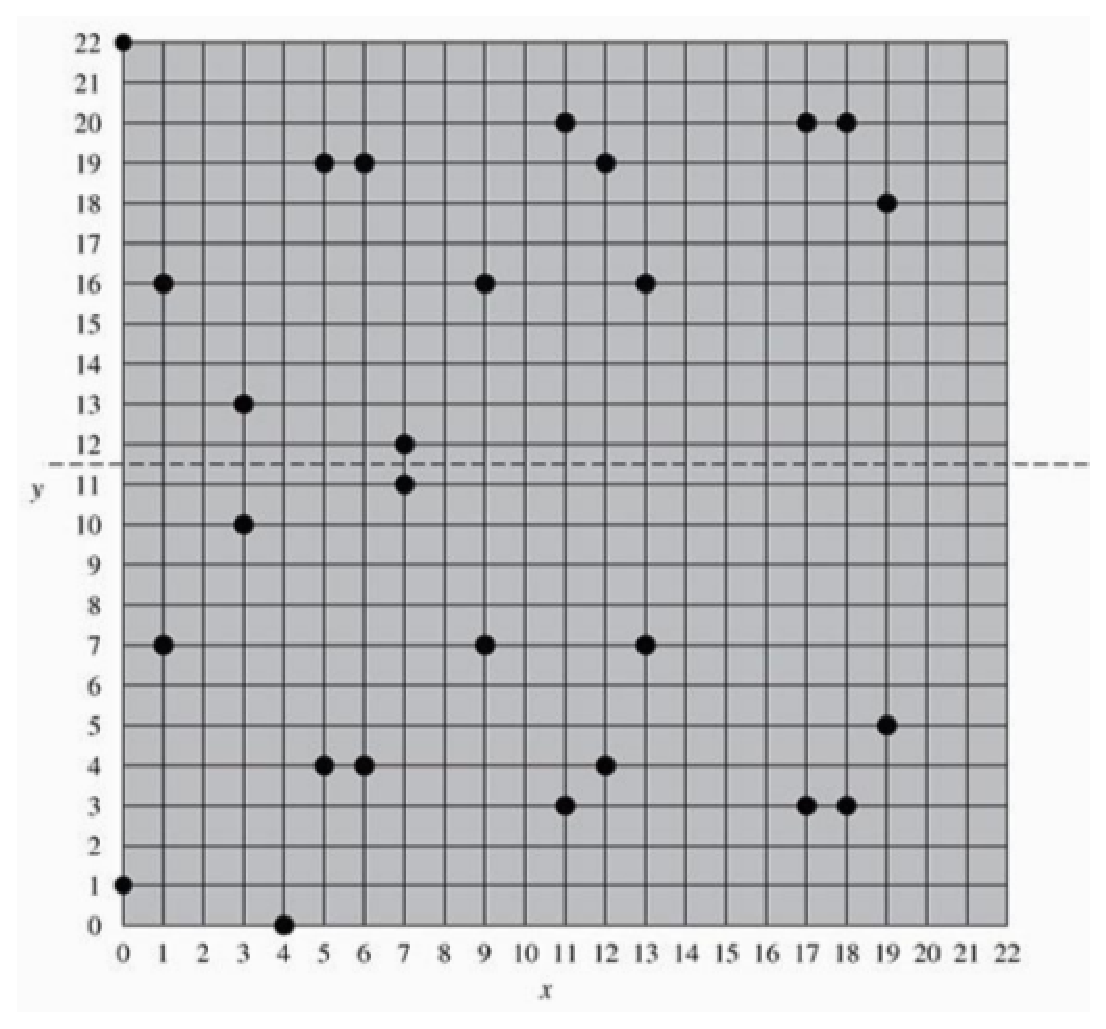
\includegraphics[scale=0.6, bb=0 0 515 478]{figuras/curva_sobre_corpo_finito.eps}
\caption{Curva elíptica $E_{23}(1, 1)$}
\label{fig:curvas}
\end{figure}

%
% CRIPTOGRAFIA DE CURVAS ELÍPTICAS
%
\subsection{Criptografia de curvas elípticas}
